\documentclass[12pt]{article}
%\usepackage[UTF8]{ctex}
\usepackage[tc]{titlepic}
\usepackage{titlesec}
\usepackage{cite}
\usepackage{fancyhdr}
\usepackage{booktabs}
\usepackage{float} 
\usepackage{graphicx} 
\usepackage{amsmath}
\usepackage{multirow}
\usepackage{amssymb}
\usepackage{amsthm}
\usepackage{mathrsfs}
\usepackage{bm}
\usepackage{tikz}
\usepackage{comment}
\usepackage{pgfplots}
\pgfplotsset{compat=1.18}
\usetikzlibrary{arrows.meta, positioning, shapes.geometric}
\usepackage{mhchem}
\usepackage{siunitx}
\usepackage[section]{placeins}
\usepackage{caption}
\usepackage{xcolor}
\usepackage{listings}
\usepackage{hyperref}
\usepackage{graphicx}
\usepackage{geometry}
\usepackage[section]{placeins}
\geometry{a4paper,scale=0.8}
\pagestyle{fancy}
\title{1}

\lstset{
language=R,
basicstyle=\color{gray}\ttfamily\small 
}

\begin{document}
\section*{questions}
\begin{itemize}
    \item what order is more \textbf{realistic}? Seems that host movement and infection should happen simultaneously but not sure how to describe that. And may need more discussion on the definition of $B$(?)
\end{itemize}


\section{description}
Let $p$ denote fraction of infected patches and fraction of uninfected patches is $1-p$. 
\begin{figure}[H]
\centering
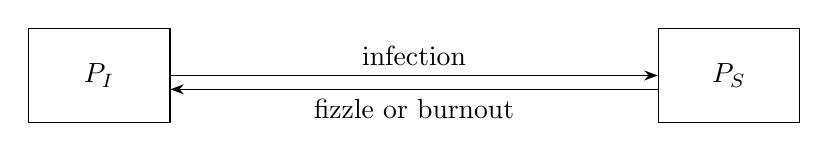
\begin{tikzpicture}[
  node distance=4cm and 3cm,
  every node/.style={align=center},
  box/.style={draw, minimum width=1.8cm, minimum height=1.2cm},
  >={Stealth}
]
% Nodes   
\node[box] (I) at (0:4) {$P_S$};  
\node[box] (S) at (180:4) {$P_I$};  
% Arrows
\draw[->] (S) -- node[above] {infection} (I);
\draw[->, transform canvas={yshift=-5pt}] (I) -- node[below] {fizzle or burnout} (S);
\end{tikzpicture}
\caption{patch state transition}
\end{figure}

Events that can cause state change:
\begin{itemize}
    \item \textbf{infection}: $\Delta p=Bp(1-p)$\\
 assuming constant $B$ 
    %$B(N_I,N_S)$ is the infection rate when average population size of infected patches is $N_I$ and average population size of uninfected patch is $N_S$. $B$ is an increasing function with respect to both. We might set
    %$$B=B_0(1-e^{-k_I N_I})(1-e^{-k_SN_S})$$
    \item \textbf{fizzle or burnout}: $\Delta p=-(1-P_1)p$\\
    where $P_1=P_1(R_0,\varepsilon,k=1,N_I)$ is persistence probability. 
    \item \textbf{migration}:
    \begin{align*}
       & N_S \leftarrow N_S-cp(N_S-N_I)\\
       & N_I \leftarrow N_I+c(1-p)(N_S-N_I)
    \end{align*}
individual rats move with probability $c$ and land in patches proportional to their availability.

    \item \textbf{epidemic}: $N_I \leftarrow (1-zD)N_I $\\
    where $z=z(R_0)$ is the final size and $D$ is the probability that an infected host dies from pathogen. 
    \item \textbf{birth}:
    \begin{align*}        
        &N_S \leftarrow N_S + rN_S(1-\frac{N_S}{K})\\
        &N_I \leftarrow N_I+ rN_I(1-\frac{N_I}{K})       
    \end{align*}
    %where $K$ is the carrying capability and $r_S$, $r_I$ are the growth rate of rats in uninfected and infected patches respectfully. (Shall we assume they are the same, or $r_I$ is smaller than $r_S$? Or shall we replace the third $N_I$ in the equation with number of healthy rats (might be approximated by $(1-z)N_I$) in infected patches?)
    \item \textbf{change of average population size when some patch state changes}: just calculate the average again after change of patch state. That is,\\

        when $\Delta p > 0$,
       $$ N_I\leftarrow\frac{pN_I+\Delta p N_S}{p+\Delta p}$$
       and $N_S$ does not change.\\

        when $\Delta p<0 $
        $$N_S\leftarrow\frac{(1-p)N_S-\Delta p N_I}{1-p-\Delta p}$$
       and $N_S$ does not change. 
\end{itemize}

To be more organized, we denote infection event with $f_i$, epidemic and burnout with $f_e$, migration with $f_m$, growth with $f_g$, then we have
$$
    f_m(p,N_I,N_S) =
    \begin{pmatrix}
        p \\
         N_I + c(1 - p)(N_S - N_I)\\
        N_S - cp(N_S - N_I) 
    \end{pmatrix} \\
$$
$$
    f_i(p,N_I,N_S) = 
    \begin{pmatrix}
        p + B(N_I,N_S)p(1 - p) \\
        \dfrac{N_I + B(1 - p)N_S}{1 + B(1 - p)}\\
        N_S 
    \end{pmatrix} \\
$$
$$
    f_e(p,N_I,N_S) =
    \begin{pmatrix}
        P_1(N_I)p \\
        (1 - zD)N_I \\
        \dfrac{(1 - p)N_S + (1 - zD)(1 - P_1)pN_I}{1 - P_1p}
    \end{pmatrix} \\
$$
$$
    f_g(p,N_I,N_S) =
    \begin{pmatrix}
        p \\
        N_I + rN_I\left(1 - \frac{N_I}{K} \right) \\
        N_S + rN_S\left(1 - \frac{N_S}{K} \right)
    \end{pmatrix}
$$
$$(p_{t+1},{N_I}_{t+1},{N_S}_{t+1})=f(p_t,N_{I_t},N_{S_t})$$

$$f=f_g  \circ f_e \circ f_i \circ f_m$$

%\textbf{The order of events has a great impact on system behavior according to the simulation(but they shouldn't… For example where should we put "migration" ).  And taking the average makes the matrix very complicated while it does not have significant biological interpretation. However I can't think of a easier or better way to deal with it…}
\section{range of parameters}
Consider quadratic function $y=x+kx(1-x)$ where $0\leq x\leq 1$ and $k\geq 0$,
$$f(x)=x+kx(1-x)=-kx^2+(k+1)x, x \in R $$

We want to make sure that $f([0,1])\subset [0,1]$. The function attains its maximum at $x^*=\frac{k+1}{2k}$. Note that $f(0)=0$ and $f(1)=1$, so we'll need to require that $x^*\geq1$, i.e. $0\leq k\leq1$. \\
\begin{itemize}
    \item \textbf{infection}:  $p\leftarrow p+Bp(1-p)$, we require $0\leq B\leq1$
    \item \textbf{burnout}: $p=P_1p$, $0\leq P_1 \leq 1$
    \item \textbf{epidemic}: $0\leq z \leq1$ and $0\leq D \leq 1$
    \item \textbf{birth}:
    \begin{align*}
         &N \leftarrow N+rN(1-\frac{N}{K}), 0\leq N \leq K\\
         \iff & x \leftarrow x+rx(1-x), 0\leq x \leq 1  \\
         &\Rightarrow 0\leq r\leq 1
    \end{align*}
\end{itemize}
When there's no infection, $(0,0)$ is an unstable equilibrium and $(K,K)$ is the only stable equilibrium, since maximum point is always greater than intersect when $r \in [0,1]$. \\
\begin{figure}[H]
    \centering
    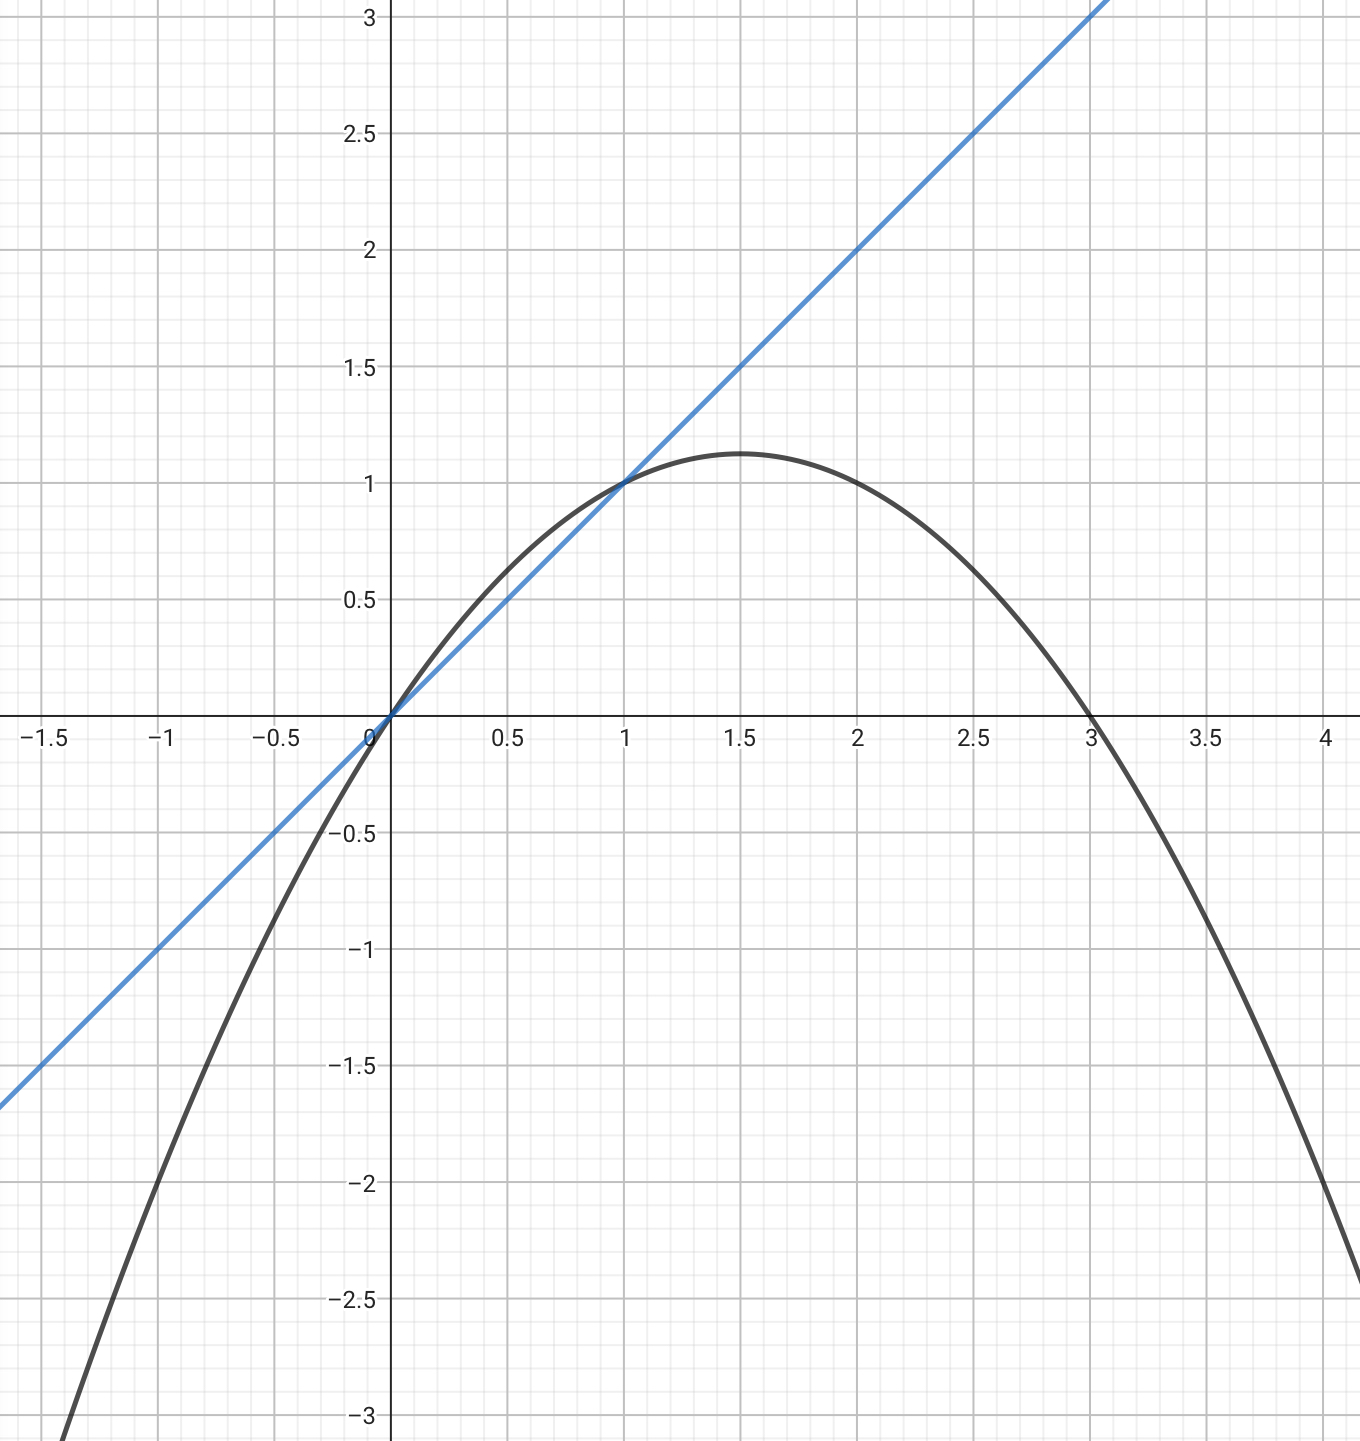
\includegraphics[width=0.7\textwidth]{Logistic.jpeg}
    \caption{logistic growth}
    \label{fig:enter-label}
\end{figure}

\begin{comment}
\begin{tabular}[H]{p{2cm}p{8cm}p{2cm}p{4cm}} 
 parameter & Definition &range &Default test value\\ 
 $B_0$& Upper bound for infection rate $B$&$[0,1]$& 0.8\\ 
 $N_0$& Initial value of average population size&$[1,+\infty)$&100\\ 
 $c_0$& migration rate&$[0,1]$&0.2\\ 
 $\varepsilon$& Mean infectious period & $(0,1)$&0.05\\ 
 $k$& Number of initially infected individuals& & 1\\ 
 $k_I$& Constant in $B$&  $(0,+\infty)$& 0.01\\ 
 $k_S$& Constant in $B$& $(0,+\infty)$& 0.01\\ 
 $r$& Birth rate& $[0,1]$& 0.1\\ 
 $K$& Carrying capacity in Logistics model&$(N_0,+\infty)$& 300\\ 
 $R_0$&basic reproduction number&$(1,\infty)$&10\\
 $p[1]$& Initial value of $p$&$[0,1]$&0.01\\ \end{tabular}
\\
\end{comment}

\section{analysis}
If we start at a point where $p>0,N_I>0,N_S>0$, it's obvious that all variables remain positive during the iterations as each step maps positive values to a positive values. \\
We want to see what happens when we start on the axes. If we set $p=0$ or $N_I=0$  then population size ends up stable at carrying capacity $K$.  $N_I=N_S=0$ means no hosts at all so nothing would happen. It's a little weird to set $N_S=0$ since it indicates that all hosts are infected, but then some would recover and the system would undergo burnout and colonization, returning to the situation that $p>0,N_I>0,N_S>0$, so we don't get anything special about that.
\begin{figure}[H]
    \centering
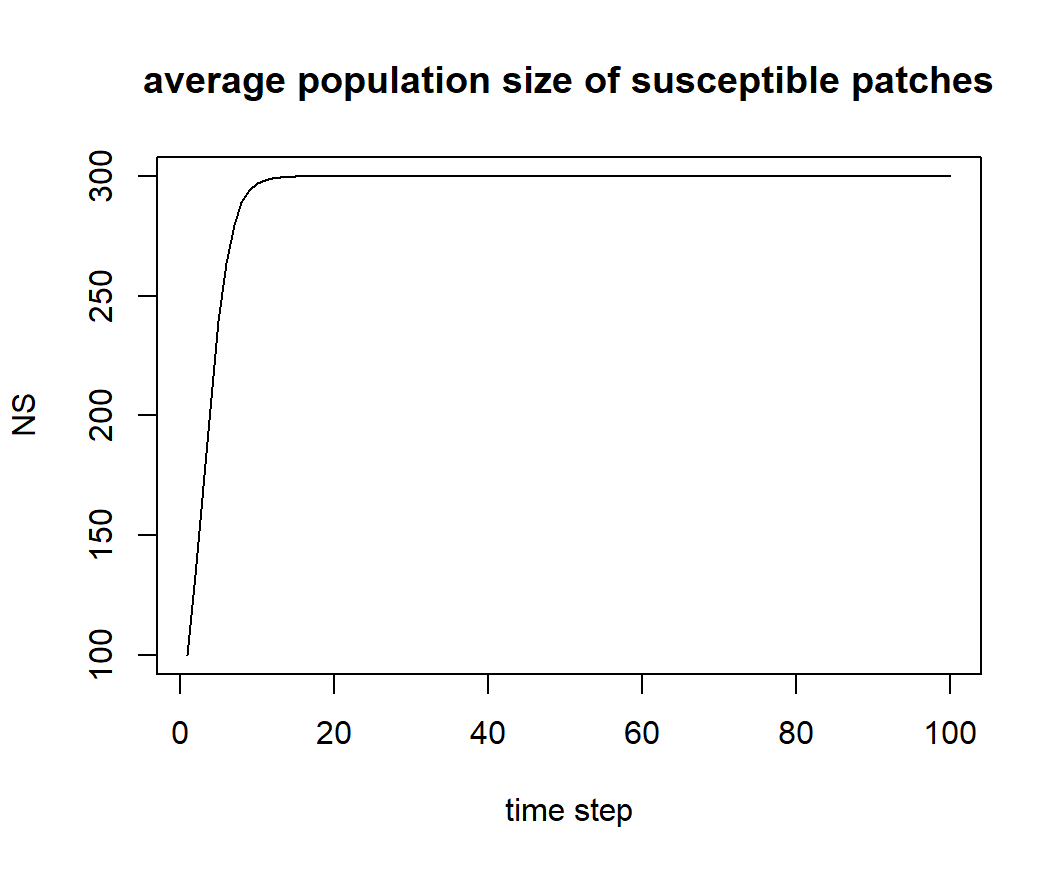
\includegraphics[width=0.8\textwidth]{DFE.png}
    \caption{DFE}
    \label{fig:enter-label}
\end{figure}

\section{invasion analysis}
$$
J_{f_m}=\begin{pmatrix}
    1&0&0\\
    -c(N_S-N_I)&1-c(1-p)&c(1-p)\\
    0&cp&1-cp
\end{pmatrix}
$$
$$J_{f_i}=\begin{pmatrix}
    1+B-2Bp&p(1-p)\frac{\partial B}{\partial N_I} &p(1-p)\frac{\partial B}{\partial N_S}\\
    -\frac{B(N_S-N_I)}{(1+B(1-p))^2}&\frac{1+B(1-p)-(N_I-N_S)(1-p)\frac{\partial B}{\partial N_I}}{(1+B(1-p))^2}& 1-\frac{1+B(1-p)-(N_I-N_S)(1-p)\frac{\partial B}{\partial N_S}}{(1+B(1-p))^2}\\
    0&0&1
\end{pmatrix}
$$

$$
J_{f_e}=\begin{pmatrix}
    P_1&p\frac{\partial P_1}{\partial N_I} &0\\
    0& 1-zD & 0\\
    J_{31}&J_{32}&\frac{1-p}{1-P_1p}
\end{pmatrix}
$$
where
\begin{align*}
&J_{31}=\frac{(-N_S+N_I(1-P_1)(1-zD))(1-P_1p)+((1-p)N_S+(1-zD)(1-P_1)pN_I)P_1}{(1-P_1p)^2}\\
&J_{32}=\frac{p(1-zD)(-\frac{\partial P_1}{\partial N_I}N_I+1-P_1)(1-P_1p)+((1-p)N_S+(1-zD)(1-P_1)pN_I)p\frac{\partial P_1}{\partial N_I}}{(1-P_1p)^2}
\end{align*}

$$
J_{f_g}=\begin{pmatrix}
    1&0&0\\
    0&1+r-\frac{2rN_I}{K}&0\\
    0&0&1+r-\frac{2rN_S}{K}
\end{pmatrix}
$$


\end{document}

